\chapter{IACTs and the Cherenkov Telescope Array}

Most modern gamma-ray observations are performed with \glspl{iact}, which are ground-based telescopes
or arrays of telescopes that use the Cherenkov light emitted by \gls{eas} in the atmosphere.
Since they are ground-based, \glspl{iact} are taking advantage of the Earth's atmosphere to get a larger
effective area than space-based instruments. This is especially true for energies above \SI{100}{\giga\eV},
\todo{confirm values} where the gamma-ray flux is low compared to lower energies. The cosmic ray flux
is shown in \autoref{fig:flux}.

% \begin{figure}
%     \centering
%     \input{build/cosmic_rays.pgf}
%     \caption{The cosmic ray flux as a function of energy. The flux is given in \si{\per\second\per\square\meter\per\steradian}.}
%     \label{fig:flux}
% \end{figure}
% \todo{PLACEHOLDER, MAYBE USE A DIFFERENT PLOT?}

The \cta{} is a new generation of \glspl{iact} that will consist of two sites,
one of which will be built at the \gls{orm} on the Canarian island of La Palma while the other site
will be built in the southern hemisphere at the \glspl{eso} Paranal Observatory in the Atacama desert
of northern Chile.

\begin{figure}
    \centering
    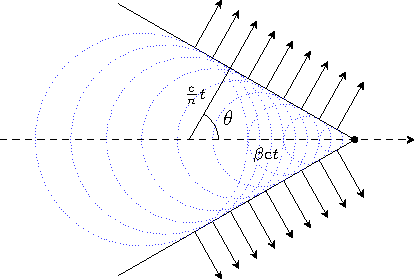
\includegraphics[width=\textwidth]{graphics/cherenkov_radiation.pdf}
    \caption{}
    \label{fig:cherenkov}
\end{figure}